% !TEX root = ../analisis.tex
\newpage

\section{Modelo de información: Consulta de Profesores}

\subsection{Descripción general}

En la figura~\ref{fig:registroInfoAspirante} se muestra la estructura de información que manejará el sistema para registrar la información de los datos personales, datos del domicilio, datos de contacto e información escolar del aspirante.

\begin{figure}[htbp!]
	\begin{center}
		\fbox{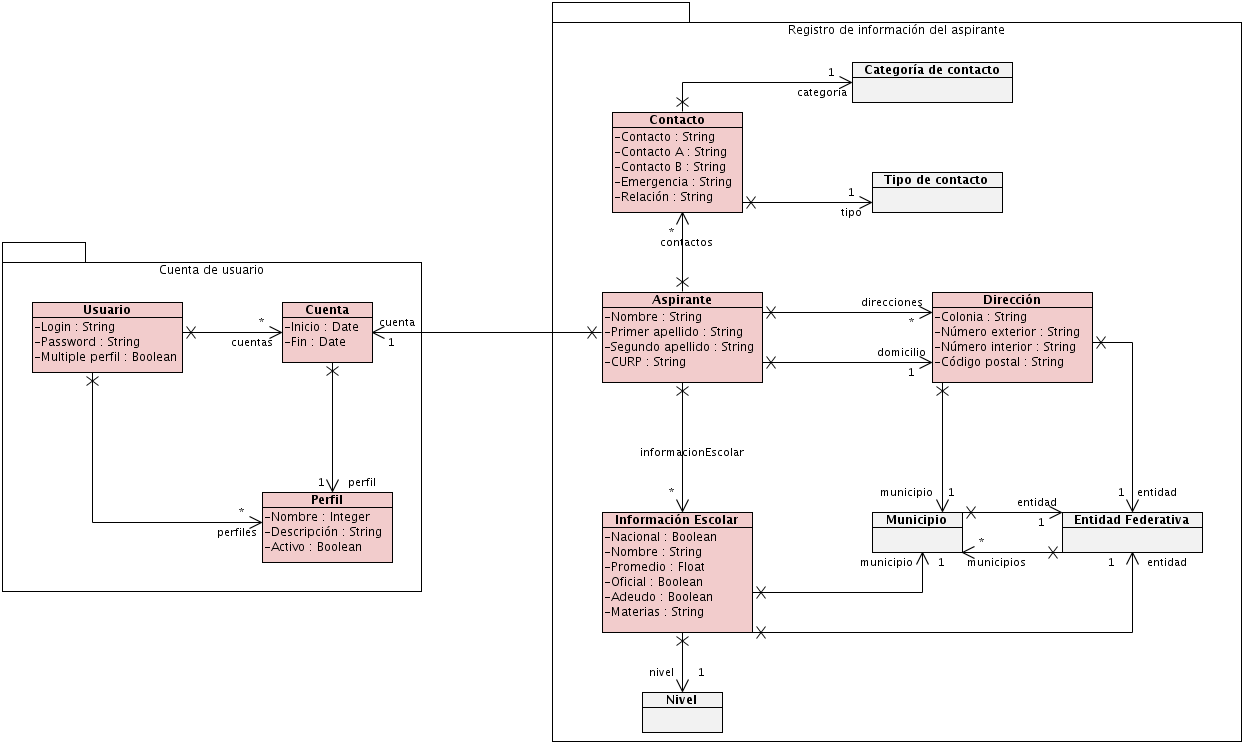
\includegraphics[width=1\textwidth]{images/clases/consulta_de_profesores}}
		\caption{Modelo de información del registro de información del aspirante.}
		\label{fig:registroInfoAspirante}
	\end{center}
\end{figure}


%--------------------------------------------------------------------------------
\begin{BusinessEntity}{Domicilio}{Domicilio}
	
	\Battr{codigoPostal}{Código postal}{\tdNumerico}{Clave numérica compuesta por cinco dígitos que identifica y ubica un domicilio}{\requerido}{\longitudExacta{5}{dígitos}}
	
	\Battr{entidadFederativa}{Entidad federativa}{\tdCatalogo}{\cdtRef{gls:entidadFederativa}{Entidad Federativa} donde está ubicado un domicilio}{\requerido}
	
	\Battr{delegacionMunicipio}{Delegación o Municipio}{\tdCatalogo}{Unidad delimitada territorialmente que pertenece a una entidad federativa donde se ubica un domicilio}{\requerido}
	
	\Battr{colonia}{Colonia}{\tdCatalogo}{Lugar que se reconoce con un nombre establecido por una norma (nombre oficial) o por la costumbre donde se ubica un domicilio}{\requerido}
	
	\Battr{calle}{Calle}{\tdFrase}{Nombre de la calle donde se ubica un domicilio}{\requerido}{\longitudMax{50}{caracteres}}
	
	\Battr{numExterior}{Número exterior}{\tdFrase}{Conjunto de caracteres alfanuméricos y símbolos que identifican a un inmueble en una vialidad}{\requerido}{\longitudMax{10}{caracteres}}
	
	\Battr{numInterior}{Número interior}{\tdFrase}{Conjunto de caracteres alfanuméricos y símbolos que identifican a un inmueble pertenecientes a un número exterior}{\requerido}{\longitudMax{10}{caracteres}}
	
	\Battr{privacidadDomicilio}{Privacidad de Domicilio}{\tdBooleano}{Indica si el domicilio está en calidad de privado o no}{\requerido}
	
	\Battr{tipoDomicilio}{Tipo de Domicilio}{\tdCatalogo}{Indica el \cdtRef{gls:tipoDomicilio}{tipo de domicilio}}{\requerido}

\end{BusinessEntity}

%--------------------------------------------------------------------------------
\begin{BusinessEntity}{InformacionEscolar}{Información Escolar}
	
	\Battr{estudioNacional}{Estudiso a nivel nacional}{\tdBooleano}{Indica si el estudio de un nivel escolar se realizó en México}{\requerido}
	
	\Battr{nombre}{Nombre de la escuela}{\tdFrase}{Nombre oficial de una escuela}{\requerido}{\longitudMax{100}{caracteres}}
	
	\Battr{promedio}{Promedio}{\tdDecimal}{Promedio que se encuentra explícito en el certificado de un nivel escolar, contiene un decimal}{\requerido}{\longitudMax{3}{dígitos}}
	
	\Battr{tipoEscuela}{Tipo de escuela}{\tdCatalogo}{Especifica el \cdtRef{gls:tipoEscuela}{tipo de escuela}}{\requerido}
	
	\Battr{adeudoMaterias}{Adeudo de materias}{\tdBooleano}{Indica si se adeudan materias a nivel bachillerato}{\requerido}
	
	\Battr{materiasAdeudadas}{Materias adeudadas}{\tdParrafo}{Son los nombres de las materias que aún están pendientes por aprobar}{\opcional}{\longitudMax{500}{caracteres}}
	
	\Battr{certificado}{Certificado de estudios}{\tdArchivo}{Es el documento que avala la información de la escuela así como el promedio obtenido en dicha escuela de una persona}{\requerido}
	
	\Battr{promedioGeneral}{Promedio General}{\tdDecimal}{Promedio global que se calcula sumando el resultado de las ponderaciones de las calificaciones de los criterios establecidos en la convocatoria, contiene un decimal}{\requerido}{\longitudMax{3}{dígitos}}
	
\end{BusinessEntity}

%--------------------------------------------------------------------------------
\begin{BusinessEntity}{Contacto}{Contacto}
	
	\Battr{medioContacto}{Medio de contacto}{\tdCatalogo}{Se refiere al \cdtRef{gls:medioContacto}{tipo de contacto}}{\requerido}
	
	\Battr{categoria}{Categoría}{\tdCatalogo}{Se refiere a la \cdtRef{gls:categoriaContacto}{clasificación del medio de contacto}}{\requerido}
	
	\Battr{fijo}{Teléfono fijo}{\tdNumerico}{Es una secuencia de dígitos que representan un número telefónico}{\requerido}{\longitudMinMax{7}{dígitos}{8}{dígitos}}
	
	\Battr{celular}{Teléfono celular}{\tdNumerico}{Es una secuencia de dígitos que representan un número telefónico móvil}{\requerido}{\longitudExacta{10}{dígitos}}
	
	\Battr{correo}{Correo electrónico}{\tdCorreo}{Es una cuenta de correo electrónico}{\requerido}{\longitudMax{250}{caracteres}}
	
	\Battr{lada}{Lada}{\tdNumerico}{Es el código del área donde pertenece el teléfono o celular}{\requerido}{\longitudMinMax{2}{dígitos}{3}{dígitos}}
	
	\Battr{extension}{Extensión}{\tdNumerico}{Es una secuencia de dígitos que representan la extensión del teléfono}{\opcional}{\longitudMax{5}{dígitos}}
	
	\Battr{emergencia}{Contacto de emergencia}{\tdFrase}{Es el nombre completo del propietario del medio de contacto de emergencia}{\requerido}{\longitudMax{50}{caracteres}}
	
	\Battr{parentesco}{Parentesco}{\tdPalabra}{Es el parentesco con la persona propietaria del medio de contacto de emergencia}{\requerido}{\longitudMax{50}{caracteres}}
	
	\Battr{privacidadDeMedioDeContacto}{Privacidad}{\tdBooleano}{Especifica si el medio de contacto se autoriza en calidad de privado o no}{\requerido}
	
\end{BusinessEntity}
